\chapter{\textgreek{Μονάδες Μετα-Επεξεργασίας}}

\pagestyle{fancy}
\fancyhf{}
%\fancyhead[OC]{\leftmark}
%\fancyhead[C]{}
%\fancyhead[EC]{\rightmark}
\renewcommand{\footrulewidth}{0.5pt}
\cfoot{\thepage}

\section{\textgreek{Επισκόπηση}}
\textgreek{Το πρόβλημα με τα Συνελικτικά Δίκτυα} (CNNs) \textgreek{είναι η προσαρμογή σε συνελικτικά φίλτρα με μεγάλα οπτικά πεδία όπως έχουμε και στην δική μας εργασία με τα διαφορετικά οπτικά πεδία που εφαρμόζονται στην παράλληλη μονάδα επεξεργασίας. Συνεπώς παράγουν χονδροειδείς εξόδους όταν αναδιαρθρώνονται για να παράγουν προβλέψεις σε επίπεδο εικονοστοιχείων και καταλήγουμε να έχουμε πιο γενικά όρια από ότι θα περιμέναμε. Επίσης, τα} CNNs \textgreek{δεν έχουν περιορισμούς ομαλότητας. Για να μπορέσουμε να διευθετήσουμε αυτό το πρόβλημα υιοθετήθηκαν δύο διαφορετικές προσεγγίσεις που θα εξηγήσουμε λεπτομερώς στα επόμενα τμήματα. Πρώτον ο αλγόριθμος Μέσου Φίλτρου που προσαρμόστηκε ως μονάδα μετα-επεξεργασίας και ο αλγόριθμος των Υποθετικών Τυχαίων Πεδίων ως Επαναλαμβανόμενα Νευρωνικά Δίκτυα} (CRFs as RNN). 

\section{\textgreek{Μεσαίο Φίλτρο}}
\textgreek{Ο αλγόριθμος του Μεσαίου Φίλτρου είναι μια μη γραμμική τεχνική ψηφιακού φιλτραρίσματος, που συχνά χρησιμοποιείται για την απομάκρυνση του θορύβου από μια εικόνα ή ένα σήμα. Μια τέτοια μείωση θορύβου είναι ένα τυπικό στάδιο προ-επεξεργασίας για τη βελτίωση των αποτελεσμάτων της μεταγενέστερης επεξεργασίας (για παράδειγμα, ανίχνευση ακμής σε μια εικόνα). Το μεσαίο φιλτράρισμα χρησιμοποιείται ευρέως στη ψηφιακή επεξεργασία εικόνων, επειδή υπό ορισμένες συνθήκες διατηρεί τις άκρες ενώ απομακρύνει τον θόρυβο έχοντας επίσης εφαρμογές στην επεξεργασία σήματος. 
\par 
Ο λόγος που χρησιμοποιήθηκε στα πειράματα μας είναι για να επιτύχουμε μια εξομάλυνση στις στην έξοδο του συστήματος, δηλαδή στις προβλέψεις του συστήματος για τα εικονοστοιχεία. Για παράδειγμα, αν μια περιοχή της εικόνας απεικονίζει έναν δρόμο, μπορεί να υπάρχουν ορισμένα εικονοστοιχεία που να έχουν προβλεφθεί ως πεζόδρομος, τότε με αυτό το φίλτρο θα πετύχουμε την μείωση των λανθασμένων εικονοστοιχείων της περιοχής της εικόνας. Η εξίσωση }\ref{eqn:median_filter} \textgreek{μας δείχνει την γενική εξίσωση της εφαρμογής ενός φίλτρου στην εικόνα, όπου  η τιμή του εικονοστοιχείου ($\mathit{g(i,j)}$) εξαρτάται από ένα σταθμισμένο άθροισμα των εικονοστοιχείων εισόδου ($\mathit{f(i+k,j+l)}$) και $\mathit{h(k,l)}$ ονομάζεται ο πυρήνας που περιέχει τους συντελεστές του φίλτρου }\cite{szeliski2011computer}.

\begin{equation}
    \centering
    \label{eqn:median_filter}
    g(i,j) = \sum_{k,l} f(i+k,j+l)h(k,l)
\end{equation}

\textgreek{Ο αλγόριθμος παρακάτω μας δείχνει βήμα-βήμα τον αλγόριθμο του Μεσαίου Φίλτρου:}

\begin{algorithm}[H]
    \caption{\textgreek{Αλγόριθμος Μεσαίου Φίλτρου} (Median Filter) \cite{wiki:median}.}
    \label{Algo_median}
  \begin{algorithmic}[2]
    \REQUIRE $\text{Output image} [W \times H]$
    \REQUIRE $\text{Input image} [W \times H]$
    \REQUIRE $Window [K \times K]$
    \REQUIRE $edgeX \gets round(K / 2)$
    \REQUIRE $edgeY \gets round(K / 2)$
    
    \FOR{\text{$x$ from edgeX to W - edgeX} }
      \FOR{\text{$y$ from edgeY to H - edgeY}}
	\STATE $i=0$
	\FOR{\text{Fx from 0 to K}}
	    \FOR{\text{Fy from 0 to K}}
		\STATE \text{$Window[i] = \text{Input image}[x + Fx - edgeX][y + Fy - edgeY]$}
		\STATE \text{$i \gets i + 1$}
	    \ENDFOR
	\ENDFOR
	\STATE \text{sort values in Window}
	\STATE \text{\text{Output Image}[x][y] $\gets$ Window[K * K / 2]}
     \ENDFOR
    \ENDFOR
    \RETURN \COMMENT{Output Image}

  \end{algorithmic}
\end{algorithm}
\textgreek{Ένα μειονέκτημα του αλγορίθμου είναι ότι για κάθε υπολογισμό ενός εικονοστοιχείου πρέπει να ταξινομήσουμε τα στοιχεία για να πάρουμε την ενδιάμεση τιμή. Επομένως, προσθέτει υπολογιστικό κόστος καθώς προσθέτει επιπλέον $\mathit{Ο(Ν^{2}})$ πράξεις.}

\section{\textgreek{Τυχαία υπό Συνθήκη Πεδία} (CRF)}
\textgreek{Τα Τυχαία υπό Συνθήκη Πεδία }(CRF) \textgreek{παρουσιάστηκαν ως μονάδα μετά-επεξεργασίας για την βελτίωση των αποτελεσμάτων. Χρησιμοποιούνται συνήθως σε προβλήματα σημασιολογικής κατάτμησης, ενώ ανήκουν στη κατηγορία των στατιστικών μοντέλων γράφων. Στην πραγματικότητα, πριν από την έλευση των νευρωνικών δικτύων και συγκεκριμένα των Συνελικτικών} (CNN), \textgreek{τα} CRF \textgreek{αποτελούσαν την καλύτερη δυνατή προσέγγιση σε θέματα σημασιολογικής κατάτμησης, ενώ πλέον χρησιμοποιούνται για βελτίωση αποτελεσμάτων καθώς τείνουν να βελτιώνουν την διαγράμμιση των ορίων των αντικειμένων στις εικόνες. Στην πραγματικότητα τα} CRF \textgreek{είναι ένα Τυχαίο Πεδίο} Markov (MRF) \textgreek{όπου οι συντελεστές του καθορίζονται από κάποιες συνθήκες στα δεδομένα.}


\subsection{\textgreek{Επισκόπηση Αλγορίθμου}}
\textgreek{Στην πραγματικότητα υπάρχουν πολλές παραλλαγές τέτοιων μοντέλων. Εμείς θα ασχοληθούμε με τα πυκνά μοντέλα} CRF \textgreek{και στην προκειμένη περίπτωση μια υλοποίηση που είναι βασισμένη σε επαναλαμβανόμενα νευρωνικά δίκτυα} (CRF as RNN). \textgreek{Θα δώσουμε μία συνοπτική περιγραφή του αλγορίθμου πριν προχωρήσουμε στην ανάλυση του. Τα }CRF \textgreek{όπως αναφέραμε, χρησιμοποιούνται για πρόβλεψη των εικονοστοιχείων, μοντελοποιούν τα εικονοστοιχεία ως τυχαίες κατανομές που δημιουργούν ένα }MRF \textgreek{όταν υπόκεινται σε μια μεγάλη κλίμακα παρατηρήσεων. Στην προκειμένη περίπτωση η μεγάλη κλίμακα παρατηρήσεων είναι η εικόνα. 
\par 
Ας υποθέσουμε ότι $X_{i}$ είναι μια τυχαία μεταβλητή που σχετίζεται με το εικονοστοιχείο $i$ το οποίο μπορεί να πάρει οποιαδήποτε τιμή από ένα σύνολο τιμών που ανήκει στο $\mathcal{L}$. Αν υποθέσουμε ότι $\mathbf{X}$ είναι το διάνυσμα των τυχαίων μεταβλητών $X_1,X_2,\dotsc,X_N$ όπου Ν ο αριθμός των εικονοστοιχείων της εικόνας. 
\par

Παίρνοντας σαν δεδομένο τον γράφο $\mathit{G = (V,E)}$ όπου $\mathit{V = {X_1,X_2,\dotsc,X_N}}$, μία παρατήρηση της εικόνας $\mathbf{I}$, το ζευγάρι $\mathbf{(I,X)}$ μπορεί να μοντελοποιηθεί ως μια κατανομή }Gibbs \textgreek{της μορφής $\mathit{P}(\mathbf{X}=\mathbf{x}|\mathbf{I}) = \frac{1}{Z(\mathbf{I})}\exp(-\mathit{E}\mathbf(x|I))$. Η συνάρτηση $\mathit{E(x)}$ είναι η ενέργεια των παρατηρήσεων $x \in \mathcal{L}^{N}$, ενώ η $Z(I)$ είναι η συνάρτηση διαμέρισης} (partition function) \cite{partition_func}. \textgreek{Στα πλήρως συνδεδεμένα }CRF \textgreek{ζεύγους }\cite{fully_crf} \textgreek{η ενέργεια της ανάθεσης ενός εικονοστοιχείου σε μια κατηγορία $\mathbf{x}$ δίνεται από την εξίσωση }\ref{eqn:energy}.

\begin{equation}
    \centering
    \label{eqn:energy}
    E(\mathbf{x}) = \sum_{i} \psi_{u}(x_{i}) + \sum_{i<j} \psi_{p}(x_{i},x_{j})
    %Q_{i}(l) \gets \frac{1}{Z_{i}} \exp(U_{i}(l))  \qquad \triangleright \text{Initialization} 
\end{equation}

\textgreek{Όπου $\psi_{u}(x_{i})$ είναι οι ενιαίοι συντελεστές ενέργειας οι οποίοι μετράνε την αντίστροφη πιθανότητα του εικονοστοιχείου $i$ να παίρνει την ετικέτα $x_{i}$ και οι συντελεστές ενέργειας ζεύγους $\psi_{p}(x_{i},x_{j})$ μετράνε το κόστος της ανάθεσης της τιμής $x_{i},x_{j}$ στα εικονοστοιχεία $i,j$ ταυτόχρονα.}

\begin{equation}
\centering
 \psi_{p}(x_{i},x_{j}) = \mu(x_{i},x_{j}) \displaystyle\sum_{m=1}^{M} w^{(m)}k_{G}^{(m)}(\mathbf{f}_{i},\mathbf{f}_j)
\end{equation}

\textgreek{Όπου $Κ_{G}^{(m)}$ (εξίσωση }\ref{eqn:gauss_kernel}) \textgreek{συνάρτηση η οποία αποτελείται από δύο Γκαουσιανύς Πυρήνες }(Gaussian Kernels) \textgreek{οι οποίοι εφαρμόζονται στα διανύσματα των στοιχείων }$\mathbf{f}_{i},\mathbf{f}_{j}$ \textgreek{τα οποία προέρχονται από τα χαρακτηριστικά της εικόνας, όπως πληροφορία θέσης των εικονοστοιχείων $(p)$ και τις τιμές των εικονοστοιχείων ($I$: }RGB values) \textgreek{και $w^{(m)}$ είναι τα βάρη των πυρήνων. Ο πρώτος πυρήνας εξαρτάται από την θέση και την τιμή των εικονοστοιχείων ενώ ο δεύτερος εξαρτάται αποκλειστικά από την θέση των εικονοστοιχείων. Οι παράμετροι $\theta_a$, $\theta_\beta$ και $\theta_\gamma$ χρησιμοποιούνται για την κανονικοποίηση των τιμών των πυρήνων. Η συνάρτηση $\mu(.,.)$ ονομάζεται συνάρτηση συμβατότητας, η οποία βρίσκει την συμβατότητα μεταξύ ενός ζεύγους εικονοστοιχείων ανάλογα με την ετικέτα που έχει ανατεθεί. Μειώνοντας την συνάρτηση ενέργειας παίρνουμε την πιο πιθανή τιμή (ετικέτα) στο $x$ δεδομένου μιας εικόνας. }

\begin{equation}
\label{eqn:gauss_kernel}
 k(\mathbf{f}_i,\mathbf{f}_j) = w^{(1)}\exp(-\frac{|p_i-p_j|^2}{2\theta^2_a }-\frac{|I_i-I_j|^2}{2\theta_\beta^2})+w^{(2)} \exp(-\frac{|p_i-p_j|^2}{2\theta^2_\gamma })
\end{equation}


\textgreek{Η εύρεση της ακριβής ελάχιστης τιμής δεν είναι εύκολο να υπολογιστεί καθώς δεν μπορούμε να υπολογίσουμε εύκολα την συνάρτηση διαμέρισης. Για αυτό τον σκοπό εφαρμόζεται η προσέγγιση Μέσου Πεδίου} (Mean-Field Approximation) \textgreek{στην κατανομή του }CRF, \textgreek{η παραπάνω διαδικασία γίνεται με την προσέγγιση της κατανομής $P(\mathbf{X})$ από μια απλούστερη κατανομή $Q(\mathbf X)$ η οποία μπορεί να γραφτεί σαν ένα γινόμενο ανεξάρτητων περιθωριακών κατανομών }$Q(\mathbf X) = \prod_{i} Q_{i}(X_{i})$. \textgreek{Παρακάτω θα δείξουμε αναλυτικά τα βήματα του αλγορίθμου και πως ο αλγόριθμος Μέσου Πεδίου μπορεί να αναδιαμορφωθεί σαν μια σειρά από πράξεις ενός ΣΝΔ (εικόνα} \ref{fig:cnn_mean_img})\textgreek{ και πως μοντελοποιείται σαν ένα ENΔ} (RNN) \cite{crf_as_rnn}.

\begin{figure}[H]
 \centering
 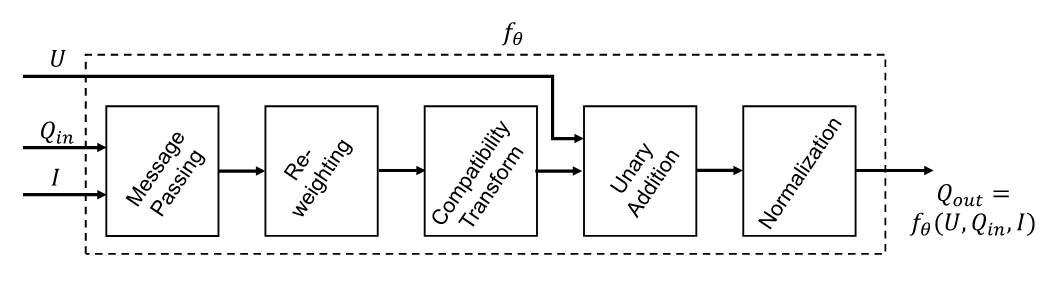
\includegraphics[scale=0.4]{Images/cnn_stack}
 \caption[MeanField as CNN]{\textgreek{Μία επανάληψη Μέσου Πεδίου ως }CNN \cite{crf_as_rnn}}
  \label{fig:cnn_mean_img}
\end{figure}

\subsection{\textgreek{Αρχικοποίηση}}
\textgreek{Στο πρώτο βήμα της αρχικοποίησης παρατηρούμε ότι στην ουσία έχουμε την εφαρμογή μιας συνάρτησης} softmax \textgreek{όπου } $Z_{i} = \sum_{l} exp(U_{i}(l))$ \textgreek{πάνω στις ενιαίες πιθανότητες} (Unary potentials). 
\\
\begin{equation}
    \label{init}
    \centering
    Q_{i}(l) \gets \frac{1}{Z_{i}} \exp(U_{i}(l))  \qquad \triangleright \text{Initialization} 
\end{equation}\\[1cm]

\subsection{\textgreek{Πέρασμα Μηνυμάτων}}
\textgreek{Στα πυκνά μοντέλα }CRF \textgreek{το πέρασμα μηνυμάτων πραγματοποιείται εφαρμόζοντας $M$ Γκαουσιανά Φίλτρα στις $Q$ κατανομές. Οι συντελεστές των φίλτρων προέρχονται από τα χαρακτηριστικά της εικόνας, όπως οι θέσεις και οι τιμές των εικονοστοιχείων, αλλά και πόσο έντονα ένα εικονοστοιχείο συσχετίζεται με ένα άλλο εικονοστοιχείο της εικόνας καθώς είναι όλα συνδεδεμένα μεταξύ τους. Επειδή ο υπολογισμός μεγάλων διαστάσεων Γκαουσιανών Φίλτρων είναι υπερβολικά μεγάλος, γίνεται η χρήση ενός αντιμεταθετικού πλέγματος} (Permutohedral lattice) \cite{lattice} \textgreek{το οποίο κάνει τον υπολογισμό των φίλτρων σε $O(N)$ χρόνο, όπου $N$ είναι το πλήθος των εικονοστοιχείων της εικόνας.} 
\par
\textgreek{Κατά τη διάρκεια της προς τα πίσω διάδοσης σφάλματος, οι είσοδοι των φίλτρων υπολογίζονται με την αποστολή των παραγώγων σφάλματος ως προς την έξοδο του φίλτρου μέσα από τα $M$ Γκαουσιανά Φίλτρα που θέσαμε αλλά με αντίστροφη κατεύθυνση. 
Επίσης, στο πλέγμα μία πολυδιάστατη συνέλιξη μπορεί να υλοποιηθεί ως μια ακολουθία από μονοδιάστατες συνελίξεις κατά μήκος των αξόνων του πλέγματος. Με αυτόν τον τρόπο το αντιμεταθετικό πλέγμα πετυχαίνει έναν πολύ αποδοτικό τρόπο περάσματος μηνυμάτων ανάμεσα στα εικονοστοιχεία.}

\begin{equation}
    \label{message}
    \centering
    %\tilde{Q}_{i}^{(m)}(l) \gets \sum_{j\neq i}
    \tilde{Q}_{i}^{(m)}(l) \gets \sum_{j\neq i} k^{(m)}(\mathbf{f}_{i},\mathbf{f}_{j})Q_{j}(l)  \qquad \triangleright \text{Message Passing} 
\end{equation}
\\[1cm]


\subsection{\textgreek{Στάθμιση Εξόδου Φίλτρου}}
\textgreek{Το επόμενο βήμα στον αλγόριθμο μέσου πεδίου λαμβάνει ένα σταθμισμένο άθροισμα των $Μ$ εξόδων φίλτρου από το προηγούμενο βήμα για κάθε ετικέτα κλάσης $l$. Όταν λαμβάνεται υπόψη κάθε ετικέτα κλάσης μεμονωμένα, μπορεί να θεωρηθεί ως μια συνέλιξη με μέγεθος φίλτρου 1 $\times$ 1 με $Μ$ κανάλια εισόδου και ένα κανάλι εξόδου. Επειδή και οι είσοδοι και οι έξοδοι σε αυτό το βήμα είναι γνωστές κατά τη διάρκεια της προς τα πίσω διάδοσης, η διαφορά σφάλματος ως προς τα βάρη του φίλτρου μπορεί να υπολογιστεί, καθιστώντας δυνατή την αυτόματη εκμάθηση των βαρών του φίλτρου.
\par 
Η παράγωγος του σφάλματος ως προς τις εισόδους μπορούν επίσης να υπολογιστούν με τον ίδιο τρόπο, να περάσουν οι παράγωγοι του σφάλματος προς τα πίσω, μέχρι το πρώτο στάδιο. Για να αποκτήσουμε μεγαλύτερο αριθμό ρυθμιζόμενων παραμέτρων, χρησιμοποιούμε ανεξάρτητα βάρη πυρήνα για κάθε ετικέτα κλάσης. Ο χωρικός πυρήνας και ο διμερής πυρήνας έχουν αντίθετες ιδιότητες και η συνεισφορά τους είναι σημαντική. Για παράδειγμα, οι διμερείς πυρήνες μπορεί από τη μία πλευρά να δίνουν έμφαση στην ανίχνευση ποδηλάτων καθώς η ομοιότητα των χρωμάτων είναι καθοριστική. Όμως, μπορεί να μην δίνουν σημασία για την ανίχνευση της τηλεόρασης, δεδομένου ότι οτιδήποτε βρίσκεται μέσα στην οθόνη της τηλεόρασης μπορεί να έχει πολλούς διαφορετικούς τύπους χρωμάτων.}\\[1cm]
\begin{equation}
    \label{eqn:weight}
    \centering
    %\tilde{Q}_{i}^{(m)}(l) \gets \sum_{j\neq i}
    \check{Q}_{i}(l) \gets \sum_{m} w^{(m)} \tilde{Q}_{i}^{(m)}(l)  \qquad \triangleright \text{Weighting Filter Outputs} 
\end{equation}
\\[1cm]

\subsection{\textgreek{Μετασχηματισμός Συμβατότητας}}
\textgreek{Στο βήμα Μετασχηματισμού Συμβατότητας, οι έξοδοι από το προηγούμενο βήμα (εξίσωση} \ref{eqn:weight})  \textgreek{μοιράζονται μεταξύ των ετικετών, ανάλογα φυσικά με τον βαθμό της συμβατότητας ανάμεσα στις ετικέτες. Η συμβατότητα μεταξύ των ετικετών των εικονοστοιχείων ορίζεται από την συνάρτηση $\mu(l,l')$.} \textgreek{Η οποία μαθαίνει την συμβατότητα μεταξύ δύο εικονοστοιχείων. Για παράδειγμα, η ανάθεση των ετικετών \emph{Άνθρωπος} και \emph{Ποδήλατο} έχουν μικρότερη ποινή από την ανάθεση των ετικετών \emph{ουρανός} και \emph{ποδήλατο}. Επίσης δεν ισχύει η μεταθετικότητα των ετικετών $\mu(l,l') \neq \mu(l',l)$. 
\par 
Η Συνάρτηση συμβατότητας μπορεί να θεωρηθεί ως ένα επιπλέον συνελικτικό επίπεδο όπου το μέγεθος του φίλτρου είναι $1\times1$ και ο αριθμός των καναλιών εισόδου και εξόδου είναι $L$. Μαθαίνοντας τα βάρη του φίλτρου είναι ισοδύναμο με την εκπαίδευση της συνάρτησης $\mathit{\mu}$ για τις ετικέτες των εικονοστοιχείων.}

\begin{equation}
    \label{compatible}
    \centering
    %\tilde{Q}_{i}^{(m)}(l) \gets \sum_{j\neq i}
    \hat{Q}_{i}(l) \gets \sum_{l'\in \mathcal{L}} \mu(l,l') \check{Q}_{i}(l')  \qquad \triangleright \text{Compatibility Transform} 
\end{equation}
\\[1cm]


\subsubsection{\textgreek{Πρόσθεση Πιθανοτήτων}}
\textgreek{Σε αυτό το βήμα, η έξοδος από τον Μετασχηματισμό Συμβατότητας αφαιρείται από τις ενιαίες πιθανότητες $U$. Εδώ δεν υπάρχουν παράμετροι, οπότε η διάδοση των διαφορών σφάλματος γίνεται απλά περνώντας τα από την έξοδο προς τις εισόδους.}

\begin{equation}
    \label{add}
    \centering
    \breve{Q}_{i}(l) \gets U_{i}(l) - \hat{Q}_{i}(l')  \qquad \triangleright \text{Adding Unary Potentials} 
\end{equation}
\\[1cm]

\subsection{\textgreek{Κανονικοποίηση}}
\textgreek{Τέλος όπως βλέπουμε στην εξίσωση} \ref{eqn:norm} \textgreek{έχουμε την κανονικοποίηση στο τέλος της επανάληψης όπου μπορεί να θεωρηθεί ως μια συνάρτηση} softmax \textgreek{χωρίς κάποιες παραμέτρους. Οι παράγωγοι από αυτό το βήμα περνάνε κανονικά προς την είσοδο μέσω της προς τα πίσω διάδοσης.}
\\[1cm]
\begin{equation}
    \label{eqn:norm}
    \centering
    %\tilde{Q}_{i}^{(m)}(l) \gets \sum_{j\neq i}
    {Q}_{i} \gets \frac{1}{Z_{i}} \exp(\breve{Q}_{i}(l)) \qquad \triangleright \text{Normalize} 
\end{equation}
\\[1cm]

\subsection{\textgreek{Τυχαία υπό Συνθήκη Πεδία ως Επαναλαμβανόμενα Νευρωνικά Δίκτυα} (CRF as RNN)}
\textgreek{Εδώ θα εξηγήσουμε πως η επαναληπτική διαδικασία του αλγορίθμου Μέσου Πεδίου μπορεί να μοντελοποιηθεί ως ένα Επαναλαμβανόμενο Νευρωνικό Δίκτυο. 
\par 
Χρησιμοποιούμε την $\mathit{f_{\theta}}$ για να υποδείξουμε την συνάρτηση μεταφοράς που προκύπτει από μια επανάληψη μέσου πεδίου. Δοθέντος μιας εικόνας $Ι$, καθώς και τις ενιαίες πιθανότητες $U$ και την εκτίμηση των περιθωριακών πιθανοτήτων $Q_{in}$ από την προηγούμενη επανάληψη, η επόμενη εκτίμηση των πιθανοτήτων δίνεται από τον εξής τύπο: $f_{\theta}(U,Q_{in},I)$. Το διάνυσμα $\mathbf{\theta} = \{w^{m},\mu(l,l')\}, \mu \in \{1,\cdots,M\},$ και $ l,l' \in \{l_{1},\cdots l_L\}$ αναπαριστούν τις παραμέτρους του }CRF \textgreek{που περιγράψαμε προηγουμένως.}
\par 
\textgreek{Οι επαναλήψεις του αλγορίθμου του Μέσου Πεδίου υλοποιούνται ως μια στοίβα από επίπεδα με τέτοιο τρόπο ώστε σε κάθε επανάληψη να παίρνει τις εκτιμήσεις $Q$ της προηγούμενης επανάληψης και τις ενιαίες πιθανότητες $U$ από το }CNN. \textgreek{Αυτή η διαδικασία που ακολουθείται είναι ίδια με την διαδικασία που ακολουθούν τα }RNN \textgreek{για εκπαίδευση. Οι εξισώσεις } \ref{eqn:H_eq_1}, \ref{eqn:H_eq_2} \textgreek{και} \ref{eqn:H_eq_3} \textgreek{μας δείχνουν την διαδικασία της επανεκτίμησης των πιθανοτήτων, όπου $Τ$ είναι ο αριθμός των επαναλήψεων του Μέσου Πεδίου} (Mean-Field Iterations):

%%%%%%%%%%%%%% H(t) Functions %%%%%%%%%%%%%%%%%%%5555
\begin{equation}
  H_{1}(t) = 
\begin{cases}
     softmax(U), \qquad t = 0\\
     H_{2}(t-1), \qquad 0< t \leq T
\end{cases}
\label{eqn:H_eq_1}
\end{equation}

\begin{equation}
  H_{2}(t) = f_{\theta}(U,H_{1}(t),I), \qquad 0 \leq t \leq T
 \label{eqn:H_eq_2}
\end{equation}

\begin{equation}
  Y(t) = 
\begin{cases}
     0, \qquad 0 \leq t < T\\
     H_{2}(t), \qquad t=T
\end{cases}
 \label{eqn:H_eq_3}
\end{equation}
%%%%%%%%%%%%%%%%%%%%%%%%%%%%%%%%%%%%%%%%%%%%%%%%%%%%%%%%%%%%%
\textgreek{Οι παράμετροι του μοντέλου }(CRF-RNN) \textgreek{είναι ίδιες με τις παραμέτρους του αλγορίθμου Μέσου Πεδίου και αναφέρονται ως $\mathit{\Theta}$. Επομένως, ο υπολογισμός των διαφορών του σφάλματος ως προς τις παραμέτρους είναι μια επανάληψη Μέσου Πεδίου, μπορούν να εκπαιδευτούν σαν Επαναλαμβανόμενο Νευρωνικό Δίκτυο με τον αλγόριθμο της Προς τα Πίσω Διάδοσης μέσω Χρόνου} (Back Propagation Through Time-BPTT) \cite{bptt_1, bptt_2}.

\begin{figure}[H]
 \centering
 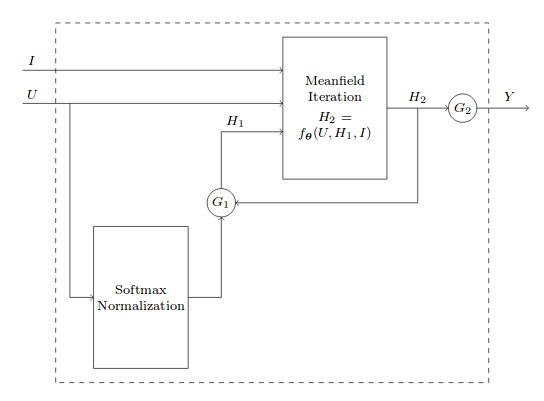
\includegraphics[scale=0.6]{Images/crf_as_rnn}
 \caption[CRF-RNN Network]{\textgreek{Ο επαναληπτικός αλγόριθμος Μέσου Πεδίου ως ένα επαναλαμβανόμενο νευρωνικό δίκτυο. Οι συναρτήσεις} $G_{1}, G_{2}$ \textgreek{είναι απλά οι συναρτήσεις εξόδου} \cite{crf_as_rnn}.}
  \label{fig:crf_rnn}
\end{figure}

\textgreek{Στην εικόνα} \ref{fig:crf-rnn-complete} \textgreek{βλέπουμε την ολοκληρωμένη αρχιτεκτονική, στο δικό μας μοντέλο οι ενιαίες πιθανότητες }(Unary potentials $\mathit U$) \textgreek{είναι η έξοδος από το τελευταίο επίπεδο του ΠΣΝΔ όπως φαίνεται στην εικόνα.}

\begin{figure}[H]
 \centering
 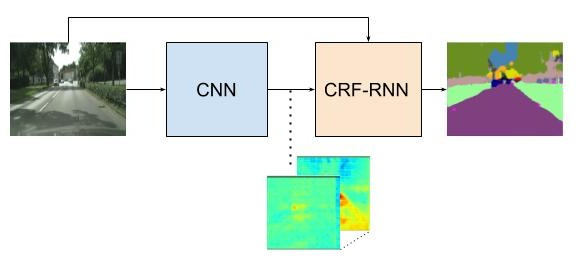
\includegraphics[scale=0.6]{Images/crf-rnn-mine}
 \caption[CNN CRF-RNN Network]{\textgreek{Ολοκληρωμένη αρχιτεκτονική του ΠΣΝΔ μαζί με το ΤΥΣΠ-ΕΝΔ. Το ΤΥΣΠ-ΕΝΔ δέχεται ως είσοδο την κανονική εικόνα μαζί με τις ενιαίες πιθανότητες του ΠΣΝΔ.}}
 \label{fig:crf-rnn-complete}
\end{figure}